\documentclass{article}
\usepackage{preamble}
\usepackage{textcomp}

\title{Using SIMBAD to Retrieve Constellation Coordinates and Brightness}
\author{Mr.~Nunez}
\date{Update on \today}

\begin{document}
\maketitle

Using the Orion constellation as an example, the following shows how to use the SIMBAD database to find the stellar coordinate and brightness information for all stars in the constellation. Go to \href{https://simbad.u-strasbg.fr/simbad/sim-fid}{https://simbad.u-strasbg.fr/simbad/sim-fid}. The screenshot below shows what the website should look like.

\begin{figure}[h!]
    \centering
    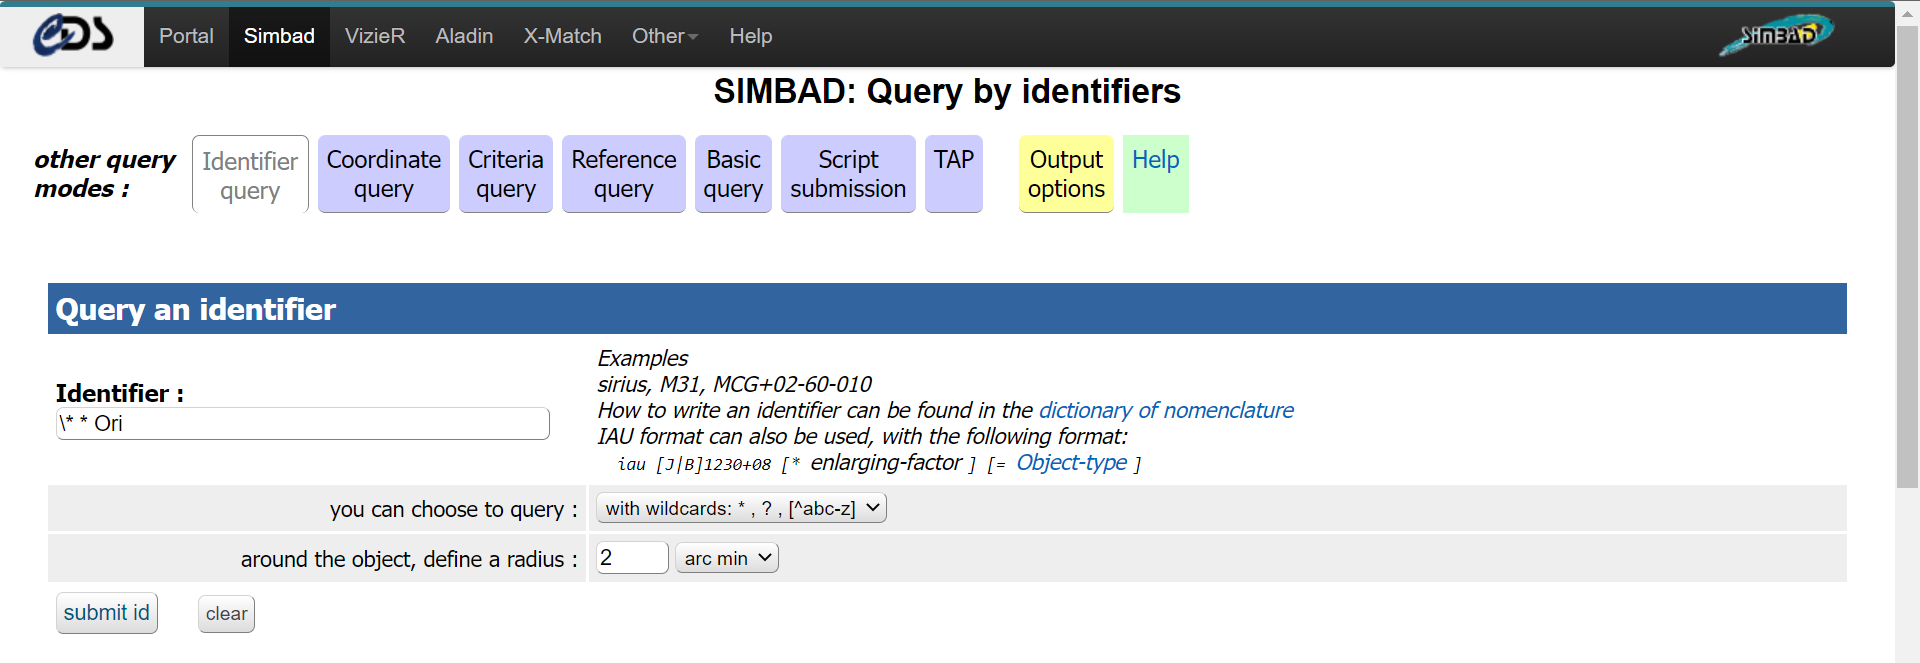
\includegraphics[width=0.8\textwidth]{Figures/SIMBAD.png}
    % \caption{Caption}
    % \label{fig:my_label}
\end{figure}

In the \texttt[red]{Identifier} box, type the following string:

\begin{center}
    \texttt{* bet Ori}
\end{center}

This query indicates that you are searching for a star (\texttt{*}) with the identifier label \texttt{bet} in the Orion (\texttt{Ori}) constellation. Clicking \texttt[red]{submit id} will reveal the page for Rigel, the blue supergiant, one of the brightest stars in Orion.

\begin{figure}[h!]
    \centering
    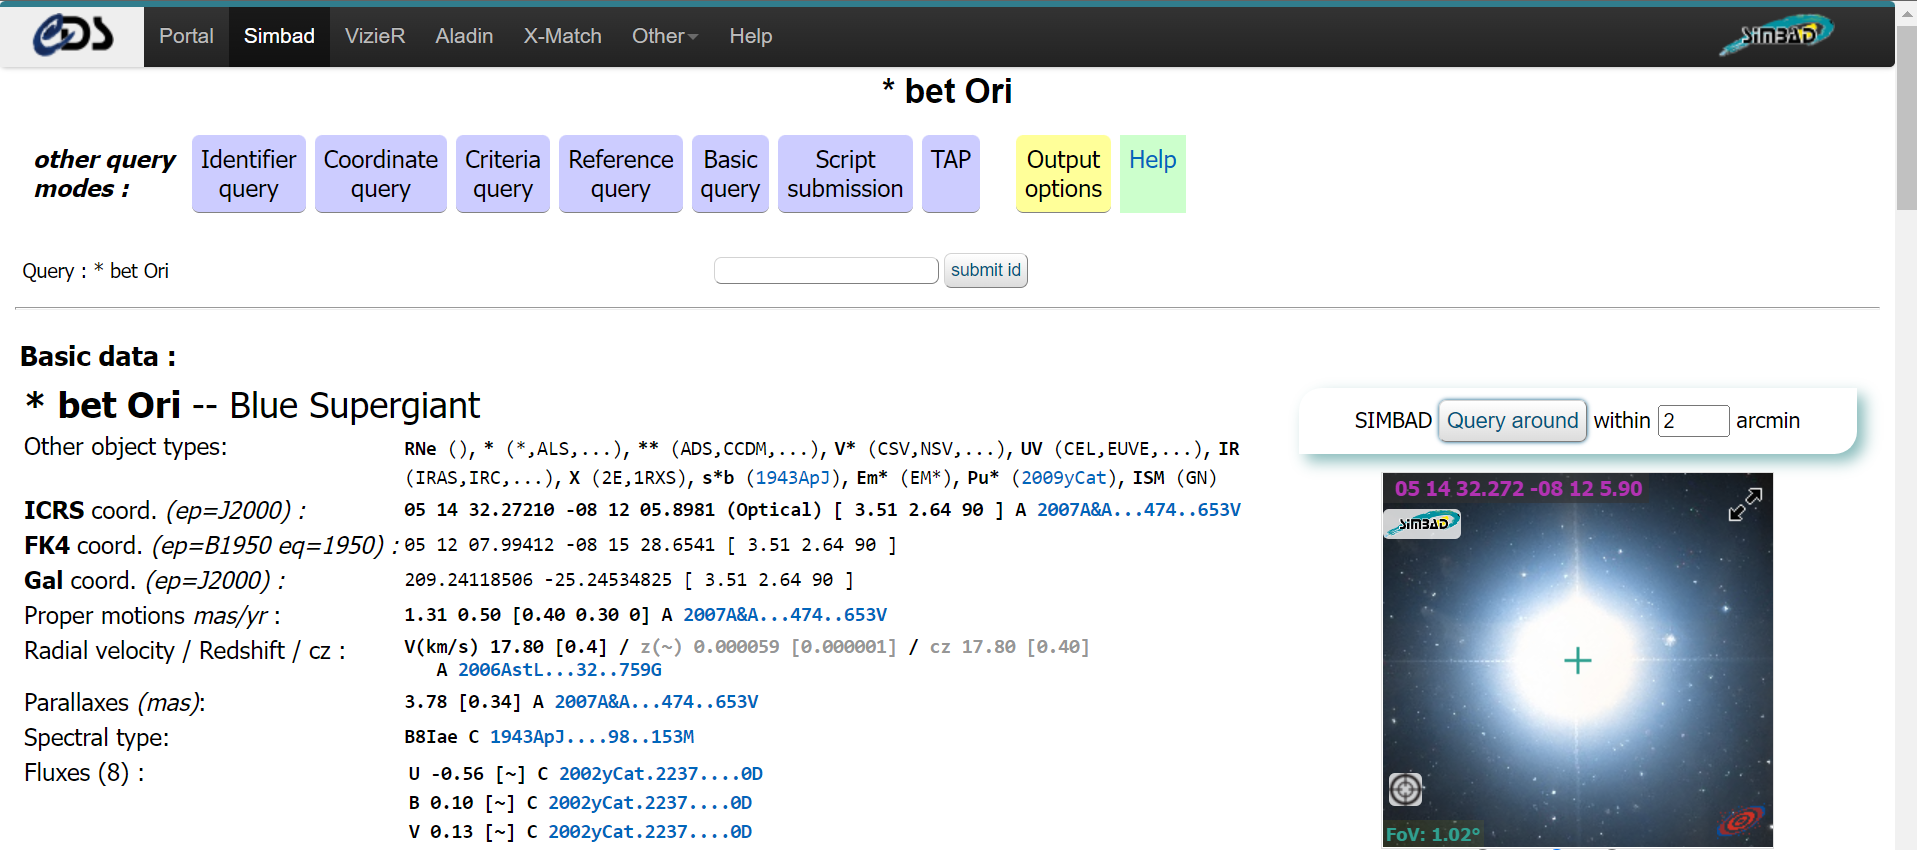
\includegraphics[width=0.7\textwidth]{Figures/Rigel.png}
\end{figure}

Next, let's see how to retrieve data for all stars in Orion. Go back to \href{https://simbad.u-strasbg.fr/simbad/sim-fid}{https://simbad.u-strasbg.fr/simbad/sim-fid}. This time, change the \texttt[red]{you can choose to query} option to \texttt[red]{with wildcards}. In the \texttt[red]{Identifier} box, enter the following string (with the spaces included): 

\begin{center}
    \texttt{\textbackslash* * Ori}
\end{center}

The \texttt{\textbackslash*} indicates you are searching for stars only. The \texttt{*} is the wildcard character, indicating that any string of characters (or empty spaces) can be included here. \texttt{Ori} is the abbreviation of the Orion constellation. Clicking \texttt[red]{submit id} will now reveal 79 rows of data pertaining to the stars that comprise the Orion region of the sky. Sorting the data table by increasing \texttt[red]{Mag V} gives you an approximate sorting of brightness to the human eye of Orion's stars, with the brightest stars on top.

\begin{figure}[h!]
    \centering
    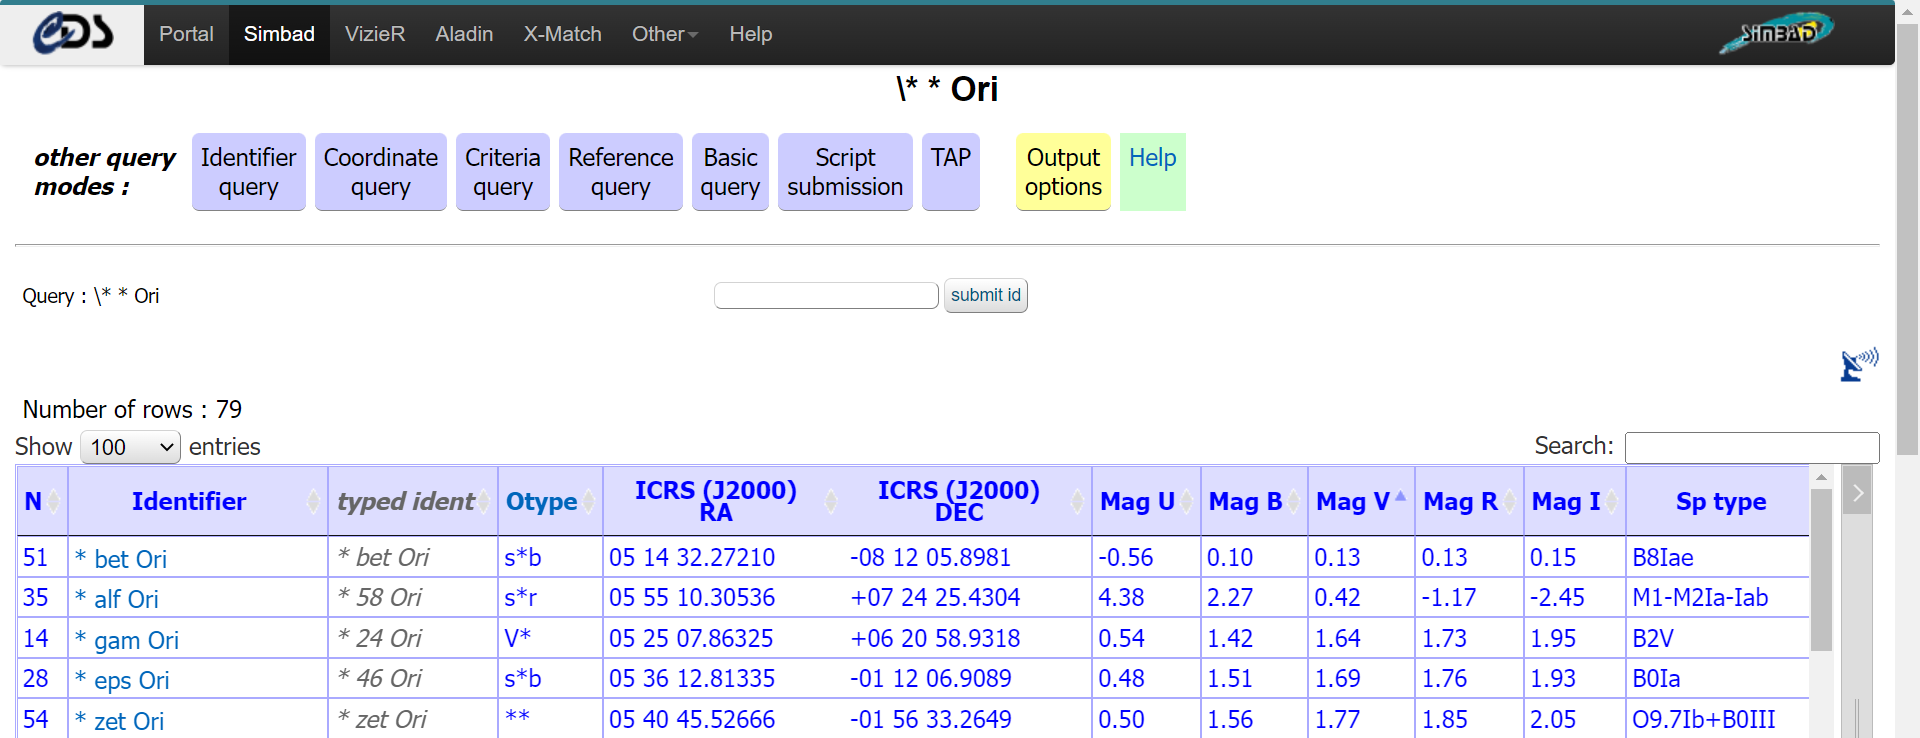
\includegraphics[width=0.7\textwidth]{Figures/Orion.png}
\end{figure}

\section{How to Plot Star Position and Brightness}

Define stellar brightness as

\begin{equation*}
    \Delta m = m_0 - m_{\star}
\end{equation*}

where $m_0$ is the apparent magnitude of the \textit{dimmest} star in the data set of a constellation and $m_{\star}$ is the apparent magnitude of each star in the constellation. This enables $\Delta m$ to serve as a proxy for the marker size in a plot. You can map each star's $\Delta m$ to its RA and DEC coordinates.

\begin{verbatim}
\addplot[%
    scatter=true,
    only marks,
    mark=*,
    point meta=explicit symbolic,
    scatter/@pre marker code/.style={/tikz/mark size=\pgfplotspointmeta/4},
    scatter/@post marker code/.style={}
] table [meta index=2] {Orion.dat};
\end{verbatim}


\end{document}